%------------------------------------------------------------------------------
% Tema 10. Models cel�lulars i animals
%------------------------------------------------------------------------------

\section{Models cel�lulars i animals}
\label{sec:models-cel.lulars-i}

Els requisits pels assajos cl�nics de ter�pia g�nica s�n:
\begin{itemize}
\item El gen ha d'estar caracteritzat i estudiat en detall.
\item S'ha de con�ixer b� la patog�nesi de la malaltia, les bases moleculars i els seus efectes.
\item Els assajos en cultiu i animals han d'haver tingut �xit.
\item Ho han d'existir ter�pies alternatives, o tractar-se de pacients refractaris a ter�pies convencionals.
\end{itemize}

Els assajos de ter�pia g�nica en models animals adients, que presenten un fenotip (simptomatologia) molt similar a la malaltia en humans, �s en molts casos imprescindible. 
Tot i aix�, l extrapolaci� de resultats no sempre �s f�cil ni directa.

Els organoides proporcionen un model d'un �rgan hum� en cultiu en condicions totalment controlades.

La mutaci� a HGPT provoca en humans un comportament autolesiu, retard mental i uric�mia. En ratol� no provoca fenotip, a no ser que tingui ADLT tamb� mutat.

L'atr�fia muscular espinal hi ha una mutaci� a SMN1. Al costat de SMN1 hi ha SMN2, que �s un pseudogen per una mutaci� puntual. Aquesta mutaci� puntual a l'ex� 7 muta un ESE (enhancer) i provoca l'skipping d'aquest ex� i es genera una prote�na sense un domini d'interacci� prote�na-prote�na. Durant la recombinaci� hom�loga, com que s�n repeticions directes es poden fusionar molt f�cilment. Un AON contra el 3' de l'ex� 7, que contenia un ESS (silencer). En un model mur�, es va injectar l'AON al ventricle cerebral i hi va haver un rescat proteic per� sense efecte fenot�pic clar. En una injecci� subcut�nia, els efectes fenot�pics es van revertir.

\begin{figure}[H]
  \centering
    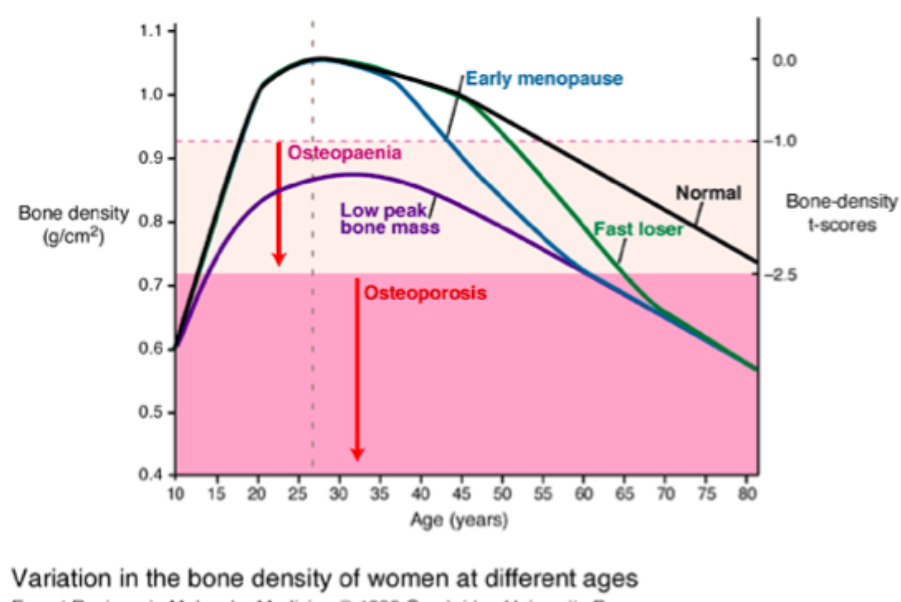
\includegraphics[width=0.85\textwidth]{fig50}
  \label{fig:fig50}
\end{figure}

\begin{figure}[H]
  \centering
    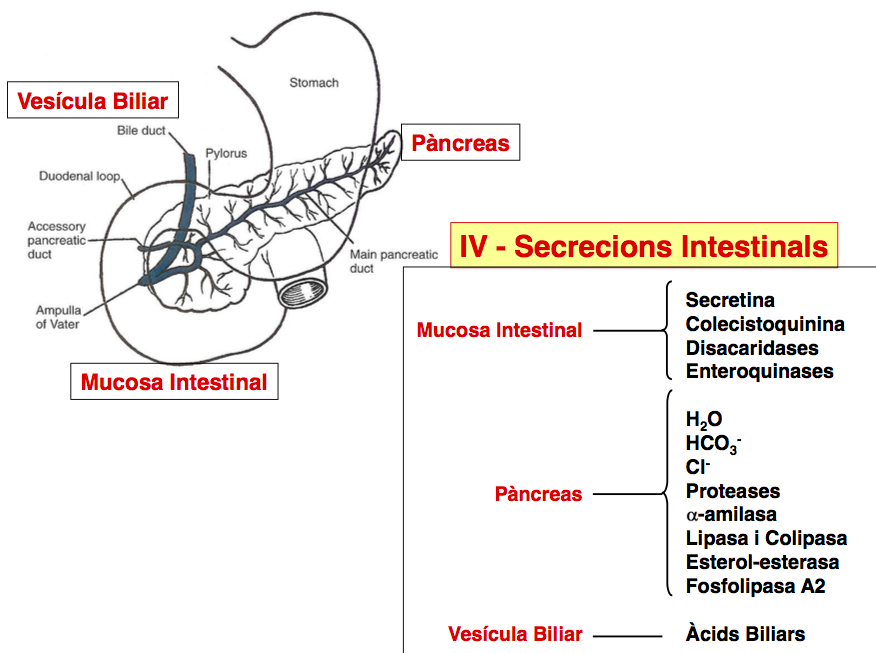
\includegraphics[width=0.85\textwidth]{fig51}
  \label{fig:fig51}
\end{figure}

Infart: van veure que VEGF controlava la regeneraci� del cor en el peix zebra. Injectaven mRNA de VEGF al lloc de l'infart. Si injectaven el DNA, es generava un cardioedema mortal. El mRNA funcionava millor.

\begin{figure}[H]
  \centering
    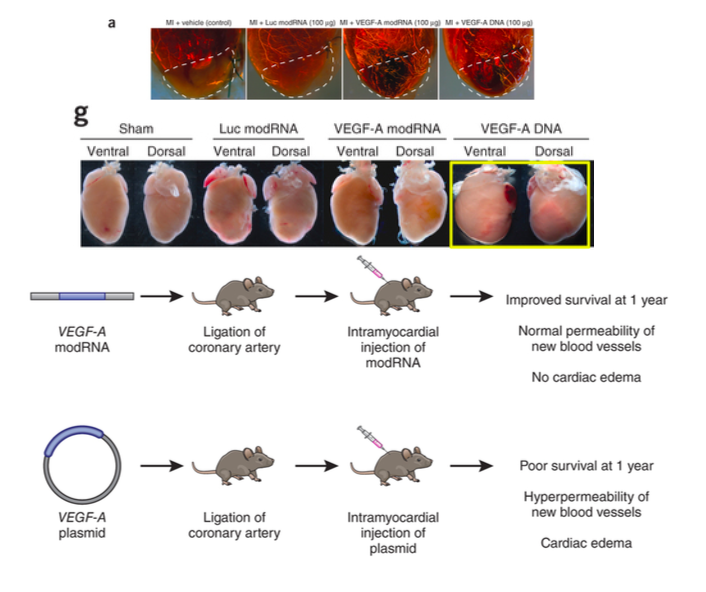
\includegraphics[width=0.85\textwidth]{fig52}
  \label{fig:fig52}
\end{figure}